\chapter{Methodology and Technologies}
  This chapter describes the methodologies in the project for the research, design, implementation and testing. It also mentions the technologies used to achieve the goals. 
  \section{Methodology} % (fold)
  \label{sec:methodology}
  This sections is basically an extension to the project plan which had to be made during the first week of the project. An approximate guideline to follow the project was set focusing on the project deadlines. I left a few weeks as margin for error in case something takes longer than planned, Figure~\ref{timline} shows the plan. 

  \begin{figure}[H]
      \centering
        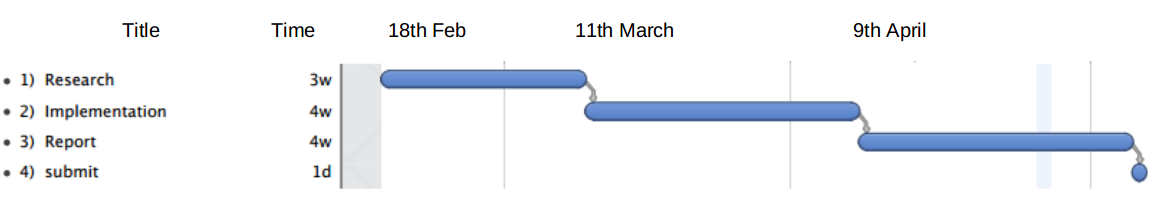
\includegraphics[width=0.9\textwidth]{time-line}
      \caption{Time line for project completion.}
      \label{timline}
  \end{figure}

  For this project to be successful I am planning on spending the initial weeks researching relevant literature and becoming familiar with the concepts of Particle Swarm Optimisation. This is a completely new field to me and understanding the key ideas and models will be critically important. Not only will I need to understand PSO's background, I will also need to study previous implementations and applications in order to become more familiar and comfortable with the algorithm. Finally, as I am planning on improving an existing algorithm, I will have to spend some time becoming familiar enough with the algorithm so that I will be able to modify it.

  The implementation stage will consist of designing the future system and the realisation of the plans. Key design decisions will have to be made during this stage and the solutions might be obtained from the analysis of previous work. 

  To complete this project I am going to test each function as I create or modified them, this will ensure a safe and stable system. This will be done to ensure that changes will not affect any previous functionality. The tests will evaluate the efficiency as well as the accuracy of my system. Given the nature of PSO's `random' initialisation of particles and their velocities,  I want to make sure that the results are consistent. 

  The writing of these result will be flexible, the sections will be written as needed or when the section arises naturally throughout the project. 

  % section methodology (end)

  \section{Technology} % (fold)
  \label{sec:technology}

    \subsection{Haskell} % (fold)
    \label{sub:haskell}
      Coming from a strong mathematical background I find functional languages easier to understand. Also one huge advantage of pure functional languages is that the absence of side-effects allow them to offer a clear semantic framework to analyse the correctness of programs. 

      As Haskell is the functional language I am most familiar with, I did not see the point in learning a new language as it would only restrict my project process, so Haskell was a clear winner. 

      There are other basic PSO implementations in other languages such as C and Ruby but as already mentioned, Haskell is my preferred language. 

    % subsection haskell (end)
    \subsection{Operating System} % (fold)
    \label{sub:operating_system}
    As Haskell is platform independent (in the sense that it can be compiled in Windows, Linux or Mac) I have chosen to use Ubuntu 12.04 as it is my preferred OS and I feel the most comfortable with it. In addition, I would not be affected in the about of software needed for the project as it is provided for all three OSs already mentioned. 

    The work was carried out on my personal laptop (Intel CORE$^{TM}$ i3 @ 2.6GHZ,4Gb RAM). If required due to any reasons, the university provides classroom PCs (Intel CORE$^{TM}$ i3-2100 CPU @3.10 GHz, 3 Gb RAM) although I have faith that my own machine will be reliable enough for me not to have to change machines. 
    
    Sublime Text 2 was chosen as the IDE for the project. It has many useful functions \cite{sublime} and similarly for the choice of OS, I am happy with this editor.
    % subsection operating_system (end)
  
  % section technology (end)
